\chapter{Functional genomics}\label{ch:bio}

\begin{quotation}
\emph{From all we have learnt about the structure of living matter, we
must be prepared to find it working in a manner that cannot be reduced
to the ordinary laws of physics - - because the construction is
different from anything we have yet tested in the physical
laboratory.}
\begin{flushright}
E. Schr{\"o}dinger (1956)
\end{flushright}
\end{quotation}

Living organisms are controlled not only by natural laws but also by
inheritable {\it genetic programs} \citep{Mayr04,Schrodinger44}. Such
{\it double causation} is a unique feature of life, and in fundamental
contrast to purely physical processes of the inanimate world. Life may
have emerged on earth more than 3.4 billion years ago
\citep{Schopf2006, Tice2004}. Genetic information evolves by means of
{\it natural selection} \citep{Darwin1859}. Living organisms maintain
homeostasis, adapt to changing environments, respond to external
stimuli, and communicate.  Peculiar features of living systems include
metabolism, growth and hierarchical organization, as well as the
ability to replicate and reproduce. All known life forms share
fundamental mechanisms at molecular level, which suggests a common
evolutionary origin of the living organisms.

The complete collection of genetic material, {\it the genome}, encodes
the heritable genetic program of an organism. Advances in measurement
technology and computational science have opened up new views to the
large-scale organization of the genome
\citep{Carroll03,Lander96}. {\it Functional genomics} is a
subdiscipline of molecular biology investigating the functional
organization and properties of genetic information. In this thesis,
new computational approaches are developed for investigation of a
central functional layer of the genome of our own species, the human
{\it transcriptome}. This chapter gives an overview to the relevant
concepts in genome biology in eukaryotic organisms and associated
genomic data resources. For further background in molecular genome
biology, see \cite{Alberts02, Brown06}.

\section{Universal genetic code}

Cells are fundamental building blocks of living organisms. All known
life forms maintain a carbon-based cellular form that carries the
genetic program \citep{Alberts02}. Each cell carries a copy of the
heritable genetic code, {\it the genome}. The human genome is divided
in 23 pairs of {\it chromosomes}, located in the nucleus of the cell,
as well as in additional mitochondrial genome. Chromosomes are
macroscopic deoxyribonucleic acid (DNA) molecules in which the DNA is
wrapped around {\it histone} molecules and packed into a peculiar {\it
  chromatin} structure that will ultimately constitute
chromosomes. The {\it genetic code} in the DNA consists of four {\it
  nucleotides}: adenosine (A), thymine (T), guanine (G), and cytosine
(C). In ribonucleic acid (RNA), the thymine is replaced by uracil
(U). Ordering of the nucleotides carries genetic information. Nucleic
acid sequences have a peculiar base pairing property, where only A-T/U
and G-C pairs can hybridize with each other. This leads to the
well-known double-stranded structure of the DNA, and forms the basis
for cellular information processing.  The \emph{central dogma of
  molecular biology} \citep{Crick70} states that DNA encodes the
information to construct proteins through the irreversible process of
{\it protein synthesis}. This is a central paradigm in molecular
biology, describing the functional organization of life at the
cellular level.

\subsection{Protein synthesis}

Genes are basic units of genetic information.  The gene is a sequence
of DNA that contains the information to manufacture a protein or a set
of related proteins. Genetic variation and regulation of gene activity
has therefore major phenotypic consequences. The {\it regulatory
  region} and {\it coding sequence} are two key elements of a
gene. The regulatory region regulates gene activity, while the coding
sequence carries the instructions for protein synthesis
\citep{Alberts02}. Interestingly, the concept of a gene remains
controversial despite comprehensive identification of the
protein-coding genes in the human genome and detailed knowledge of
their structure and function \citep{Pearson2006}.

Proteins, encoded by the genes, are key functional entities in the
cell. They form cellular structures, and participate in cell signaling
and functional regulation. {\it Protein synthesis} refers to the
cell-biological process that converts genetic information into final
functional protein products (Figure~\ref{fig:bio}A). Key steps in
protein synthesis include transcription, pre-mRNA splicing, and
translation. In {\it transcription}, the double-stranded DNA is opened
in a proximity of the gene sequence and the process is initiated on
the regulatory region of the gene. The DNA sequence of the gene is
then converted into a complementary pre-mRNA by a polymerase
enzyme. The pre-mRNA sequence contains both protein coding and
non-coding segments. These are called {\it exons} and {\it introns},
respectively. In {\it pre-mRNA splicing}, the introns are removed and
the exons are joined together to form mature {\it messenger-RNA
  (mRNA)}. A gene can encode multiple splice variants, corresponding
to different exon definitions and their combinations; this is called
{\it alternative splicing}. The mature mRNA is exported from nucleus
to the cell cytoplasm. In {\it translation} the mRNA is converted into
a corresponding amino acid sequence in ribosomes based on the {\it
  universal genetic code} that defines a mapping between nucleic acid
triplets, so-called {\it codons}, and amino acids. The code is common
for all known life forms. Each consecutive codon on the mRNA sequence
corresponds to an amino acid, and the corresponding sequence of amino
acids constitutes a protein. In the final stage of protein synthesis,
the amino acid sequence folds into a three-dimensional structure and
undergoes {\it post-translational modifications}. The structural
characteristics of a protein molecule will ultimately determine its
functional properties \citep{Alberts02}.

\begin{figure}[ht]\label{fig:bio}
\centerline{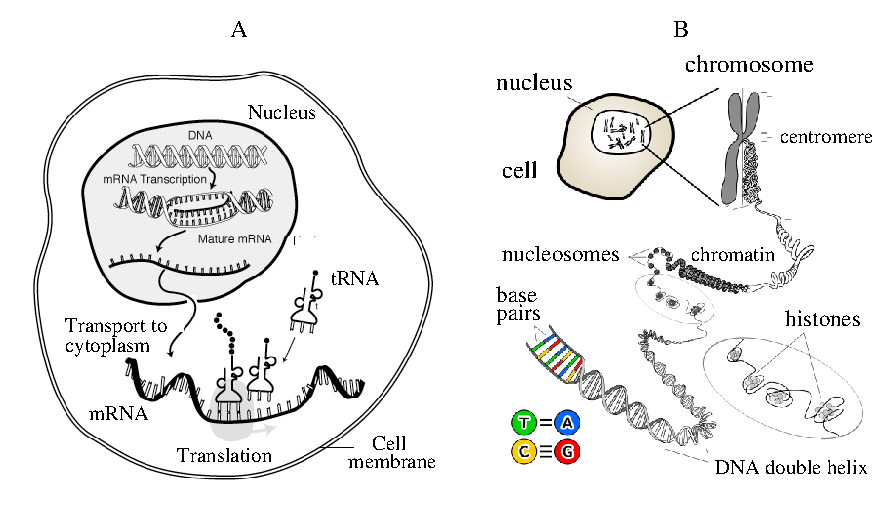
\includegraphics[width=.9\textwidth]{pic/bio.eps}}
\caption{{\bf A} Key steps of protein synthesis. The two key processes
  in protein synthesis are called {\it transcription} and {\it
    translation}, respectively. In transcription, the DNA sequence of
  the gene is transcribed into pre-mRNA based on the base pairing
  property of nucleic acid sequences. The pre-mRNA is modified to
  produce mature messenger-RNA (mRNA), which is then transported to
  cytoplasm. Transfer-RNA (tRNA) carries the mRNA to ribosomes, where
  it is translated into an amino acid sequence based on the universal
  genetic code where each nucleotide triplet of the mRNA sequence,
  so-called \emph{codon}, corresponds to a particular amino acid. The
  amino acid sequence is subsequently modified to form the final
  functional protein product. {\bf B} Organization of the genetic
  material in an eukaryotic cell. The nucleotide base pairs form the
  double helix structure of DNA. This is wrapped around histone
  molecules to form nucleosomes, and the chromatin sequence. The
  chromatin is tightly packed to form chromosomes that carry the
  genetic material and are located in the cell nucleus. The image has
  been modified from
  http://commons.wikimedia.org/wiki/File:Chromosome\_en.svg.}
\end{figure}
% Protein synthesis image:
% The image has been modified from http://en.wikipedia.org/wiki/File:MRNA-interaction.png.

\subsection{Layers of regulation}

Phenotypic changes can rarely be attributed to changes in individual
genes; cell function is ultimately determined by coordinated
activation of genes and other biomolecular entities in response to
changes in cell-biological environment \citep{Hartwell99}. Gene
activity is regulated at all levels of protein synthesis and cellular
processes. A major portion of functional genome sequence and protein
coding-genes themselves participate in the regulatory system itself
\citep{Lauffenburger00}.

{\it Epigenetic regulation} refers to chemical and structural
modifications of chromosomal DNA, the {\it chromatin}, for instance
through methylation, acetylation, and other histone-binding molecules.
Such modifications affect the packing of the DNA molecule around {\it
  histones} in the cell nucleus. The combinatorial regulation of such
modifications regulates access to the gene sequences
\citep{Gibney2010}. Epigenetic changes are believed to be heritable
and they constitute a major source of variation at individual and
population level \citep{Johnson2010}. {\it Transcriptional regulation}
is the next major regulatory layer in protein synthesis. So-called
{\it transcription factor} proteins can regulate the transcription
rate by binding to control elements in gene regulatory region in a
combinatorial fashion. {\it Post-transcriptional modifications} will
then regulate pre-mRNA splicing. Up to 95\% of human multi-exon genes
are estimated to have alternative splice variants
\citep{Pan2008}. Consequently, a variety of related proteins can be
encoded by a single gene. This contributes to the structural and
functional diversity of cell function \citep{Stetefeld2005}. Several
mechanisms will then affect {\it mRNA degradation} rates. For
instance, micro-RNAs that are small, 21-25 basepair nucleotide
sequences can inactivate specific mRNA transcripts through
complementary base pairing, leading to mRNA degradation, or prevention
of translation. Finally, {\it post-translational modifications}, {\it
  protein degradation}, and other mechanisms will affect the
three-dimensional structure and life cycle of a protein. The proteins
will participate in further cell-biological processes. The processes
are in continuous interaction and form complex functional networks,
which regulate the life processes of an organism \citep{Alberts02}.

\section{Organization of genetic information}

The understanding of the structure and functional organization of the
genome is rapidly accumulating with the developing genome-scanning
technologies and computational methods. This section provides an
overview to key structural and functional layers of the human genome.

\subsection{Genome structure}

The genome is a dynamic structure, organized and regulated at multiple
levels of resolution from individual nucleotide base pairs to complete
chromosomes (Figure~\ref{fig:bio}B; \cite{Brown06}). A major portion
of heritable variation between individuals has been attributed to
differences in the genomic DNA sequence. Traditionally, main genetic
variation was believed to arise from small point mutations, so-called
{\it single-nucleotide polymorphisms (SNPs)}, in protein-coding
DNA. Recently, it has been increasingly recognized that {\it
  structural variation} of the genome makes a remarkable contribution to
genetic variation. Structural variation is observed at all levels of
organization from single-nucleotide polymorphisms to large chromosomal
rearrangements, including deletions, insertions, duplications,
copy-number variants, inversions and translocations of genomic regions
\citep{Feuk06, Sharp06}. Such modifications can directly and
indirectly influence transcriptional activity and contribute to human
diversity and health \citep{Collins03, Hurles08}.

The draft DNA sequence of the complete human genome was published in
2001 \citep{Lander01, Venter01}. The human genome contains three
billion base pairs and approximately 20,000-25,000 protein-coding
genes \citep{Collins04}. The protein-coding exons comprise less than
1.5\% of the human genome sequence. Approximately 5\% of the human
genome sequence has been conserved in evolution for more than 200
million years, including the majority of protein-coding genes
\citep{encode07, Waterston02}. Half of the genome consists of highly
repetitive sequences. The genome sequence contains structural elements
such as centromeres and telomeres, repetitive and mobile elements,
\citep{Prak00}, retroelements \citep{Bannert04}, and non-coding,
non-repetitive DNA \citep{Collins03}. The functional role of
intergenic DNA, which forms 75\% of the genome, is to a large extent
unknown \citep{Venter01}. Recent evidence suggests that the
three-dimensional organization of the chromosomes, which is to a large
extent regulated by the intergenic DNA is under active selection, can
have a remarkable regulatory role \citep{Lieberman-Aiden2009,
  Parker2009}. Comparison of the human genome with other organisms,
such as the mouse \citep{Waterston02} can highlight important
evolutionary differences between species. For a comprehensive review
of the structural properties of the human genome, see \cite{Brown06}.


\subsection{Genome function}

In protein synthesis, the gene sequence is transcribed into pre-mRNA,
which is then further modified into mature messenger-RNA and
transported to cytoplasm. An average cell contains over 300,000 mRNA
molecules, and the mRNA concentration, or {\it expression levels} of
individual genes, vary according to Zipf's law, a power-law
distribution where most genes are expressed at low concentrations,
perhaps only one or few copies of the mRNA per cell on average, and a
small number of genes are highly expressed, potentially with thousands
of copies per cell \citep[see][]{Carninci2009, Furusawa2003}.
Cell-biological processes are reflected at the transcriptional
level. Transcriptional activity varies by cell type, environmental
conditions and time. Different collections of genes are active in
different contexts. {\it Gene expression}, or mRNA expression, refers
to the expression level of an mRNA transcript at particular
physiological condition and time point. In addition to protein-coding
mRNA molecules that are the main target of analysis in this thesis,
the cell contains a variety of other functional and non-functional
mRNA transcripts, for instance micro-RNAs, ribosomal RNA and
transfer-RNA molecules \citep{Carninci2009, Johnson05}.

The {\it transcriptome} refers to the complete collection of mRNA
sequences of an organism. This is a central functional layer of the
genome that regulates protein production in the cells, with a
significant role in creating genetic variation
\citep{Jordan05}. According to current estimates, up to 90\% of the
eukaryotic genome can be transcribed \citep{Carninci05, Gagneur2009}.
The protein-coding mRNA transcripts are translated into proteins at
ribosomes during protein synthesis. 

{\it The proteome} refers to the collection of protein products of an
organism. The proteome is a main functional layer of the genome. Since
the final protein products carry out a main portion of the actual cell
functions, techniques for monitoring the concentrations of all
proteins and their modified forms in a cell simultaneously would
significantly help to improve the understanding of the cellular
systems \citep{Collins03}. However, sensitive, reliable and
cost-efficient genome-wide screening techniques for measuring protein
expression are currently not available. Therefore genome-wide
measurements of the mRNA expression levels are often used as an
indirect estimate of protein activity.

In addition to the DNA, RNA and proteins, the cell contains a variety
of other small molecules. The extreme functional diversity of living
organisms emerges from the complex network of interactions between the
biomolecular entities \citep{Barabasi04, Hartwell99}. Understanding of
these networks and their functional properties is crucial in
understanding cell function \citep{Collins03, Schadt2009}. However,
the systemic properties of {\it the interactome} are poorly
characterized and understood due to the complexity of biological
phenomena and incomplete information concerning the interactions.  The
cell-biological processes are inherently modular \citep{Hartwell99,
  Ihmels02, Lauffenburger00}, and they exhibit complex {\it pathway
  cross-talk} between the cell-biological processes \citep{Li08c}. In
modular systems, small changes can have significant regulatory effects
\citep{Espinosa-Soto2010}.

\section{Genomic data resources}

Systematic observations from the various functional and regulatory
layers of the genome are needed to understand cell-biological
systems. Efficient sharing and integration of genomic information
resources through digital media has enabled large-scale investigations
that no single institution could afford. The public human genome
sequencing project \citep{Lander01} is a prime example of such
project. Results from genome-wide transcriptional profiling studies
are routinely deposited to public repositories \citep{Barrett2009,
  Parkinson2009}. Sharing of original data is increasingly accepted as
the scientific norm, often following explicit data release
policies. The establishment of large-scale databases and standards for
representing biological information support the efficient use of these
resources \citep{Bammler05, Brazma06}. A continuously increasing array
of genomic information is available in these databases, concerning
aspects of genomic variability across individuals, disease states, and
species \citep{Brent2008, Church05, Cochrane2010,
  G10KCOSconsortium2009, tcga08}.

\subsection{Community databases and evolving biological knowledge}
\label{sec:biodata}

\subsubsection{Genomic sequence databases}

During the human genome project and preceding sequencing projects DNA
sequence reads were among the first sources of biological data that
were collected in large-scale public repositories, such as GenBank
\citep{Benson2010}. GenBank contains comprehensive sequence
information of genomic DNA and RNA for a number of organisms, as well
as a variety of information concerning the genes, non-coding regions,
disease associations, variation and other genomic features. Online
analysis tools, such as the Ensembl Genome browser \citep{Flicek2010},
facilitate efficient use of these annotation
resources. Next-generation sequencing technologies provide rapidly
increasing sequencing capacity to investigate sequence variation
between individuals, populations and disease states
\citep{Ledford2010, McPherson2009}. In particular, the human and mouse
transcriptome sequence collections at the Entrez Nucleotide database
of GenBank are utilized in this thesis, in Publications~\ref{PECA}
and~\ref{RPA}.

\subsubsection{Transcriptome databases}

Gene expression measurement provides a snapshot of mRNA transcript
levels in a cell population at a specific time and condition,
reflecting the activation patterns of the various cell-biological
processes. While gene expression measurements provide only an indirect
view to cellular processes, their wide availability provides a unique
resource for investigating gene co-regulation on a genome- and
organism-wide scale. Versatile collections of microarray data in
public repositories, such as the Gene Expression Omnibus (GEO;
\cite{Barrett2009}) and ArrayExpress \citep{Parkinson2009} are
available for human and model organisms, and they contain valuable
information of cell function \citep{Carninci05, DeRisi97, Russ10,
  Zhang04b}.

Several techniques are available for quantitative and highly parallel
measurements of mRNA or {\it gene expression}, allowing the
measurement of the expression levels of tens of thousands of mRNA
transcripts simultaneously \citep{Bradford2010}. Microarray techniques
are routinely used to measure the expression levels of tens of
thousands of mRNA transcripts in a given sample, and transcriptional
profiling is currently a main high-throughput technique used to
investigate gene function at genome- and organism-wide scale
\citep{Gershon05, Yauk04}. Increasing amounts of transcriptional
profiling data are being produced by sequencing-based methods
\citep{Carninci2009}. A main difference between the microarray- and
sequencing-based techniques is that gene expression arrays have been
designed to measure predefined mRNA transcripts, whereas
sequencing-based methods do not require prior information of the
measured sequences, and enable {\it de novo} discovery of expressed
transcripts \citep{Bradford2010, Hoen08}. Large-scale microarray
repositories provide currently the most mature tools for data
processing and retrieval, and form the main source of transcriptome
data in this thesis.

Microarray technology is based on the base pairing property of nucleic
acid sequences where the DNA or RNA sequences in a sample bind to the
complementary nucleotide sequences on the array. This is called {\it
  hybridization}.  The measurement process begins by the collection of
cell samples and isolation of the sample mRNA. The isolated mRNA is
converted to cDNA, {\it labeled} with specific marker molecules, and
hybridized on complementary probe sequences on the array. The array
surface may contain hundreds of thousands of spots, each containing
specific probe sequences designed to uniquely match with particular
mRNA sequences. The hybridization level reflects the target mRNA
concentration in the sample, and it is estimated by measuring the
intensity of light emitted by the label molecules with a laser
scanner. {\it Short oligonucleotide arrays} \citep{Lockhart96} are
among the most widely used microarray technologies, and they are the
main source of mRNA expression data in this thesis.  Short
oligonucleotide arrays utilize multiple, typically 10-20, probes for
each transcript target that bind to different regions of the same
transcript sequence. Use of several 25-nucleotide probes for each
target leads to more robust estimates of transcript activity. Each
probe is expected to uniquely hybridize with its intended target, and
the detected hybridization level is used as a measure of the activity
of the transcript. A short oligonucleotide array measures absolute
expression levels of the mRNA sequences; relative differences between
conditions can be investigated afterwards by comparing these
measurements. A standard whole-genome array measures typically
\(\sim\)20,000-50,000 unique transcript sequences. A single microarray
experiment can therefore produce hundreds of thousands of raw
observations.

Comparison and integration of individual microarray experiments is
often challenging due to remarkable experimental variation between the
experiments. Common standards have been developed to advance the
comparison and integration \citep{Brazma01, Brazma06}. Carefully
controlled integrative datasets, so-called {\it gene expression
  atlases}, contain thousands of genome-wide measurements of
transcriptional activity across diverse conditions in a directly
comparable format. Examples of such data collections include
GeneSapiens \citep{Kilpinen08}, the human gene expression atlas of the
European Bioinformatics Institute \citep{Lukk10}, as well as the
NCI-60 cell line panel \citep{Scherf2000}. Integrative analysis of
large and versatile transcriptome collections can provide a holistic
view of transcriptional activity of the various cell-biological
processes, and opens up possibilities to discover previously
uncharacterized cellular mechanisms that contribute to human health
and disease.


\subsubsection{Other types of microarray data}

Microarray techniques can also be used to study other functional
aspects of the genome, including epigenetics and micro-RNA regulation,
chromosomal aberrations and polymorphisms, alternative splicing, as
well as transcription factor binding \citep{Butte02a, Hoheisel06}.
For instance, chromosomal aberrations can be measured with the {\it
  array comparative genome hybridization method (aCGH;}
\citealt{Pinkel2005}), which is based on hybridization of DNA sequences
on the array surface. Copy number changes are a particular type of
chromosomal aberrations, which are a major mechanism for cancer
development and progression. Copy number alterations can cause changes
in gene- and micro-RNA expression, and ultimately cell-biological
processes \citep{Beroukhim10}.  A public repository of copy number
measurement data is provided for instance by the CanGEM database
\citep{Scheinin08}. In Publication~\ref{MLSP}, microarray measurements
of DNA copy number changes are integrated with transcriptional
profiling data to discover potential cancer genes for further
biomedical analysis.

\subsubsection{Pathway and interaction databases}

Curated information concerning cell-biological processes is valuable
in both experimental design and validation of computational studies
\citep{Blake04}. Representation of dynamic biochemical reactions in
their full richness is a challenging task beyond a mere listing of
biochemical events; a variety of proteins and other compounds interact
in a hierarchical manner through various molecular mechanisms
\citep{Hartwell99, Przytycka2010}. Standardized database formats such
as the BioPAX \citep{BioPAX05} and SBML \citep{Stromback05} advance
the accumulation of highly structured biological knowledge and
automated analysis of such data. A huge body of information concerning
cell-biological processes is available in public repositories. The
most widely used annotation resources include the Gene Ontology (GO)
database \citep{Ashburner00} and the KEGG pathway database
\citep{Kanehisa2010}. The GO database provides functional annotations
for genes and can be used for instance to detect enrichment of certain
functional categories among the key findings from computational
analysis, as in Publication~\ref{AC}, where enrichment analysis is
used for both validation and interpretation purposes.  Pathways are
more structured representations concerning cellular processes and
interactions between molecular entities. Such prior information can be
used to guide computational modeling, as in Publication~\ref{NR},
where pathway information derived from the KEGG pathway database is
used to guide organism-wide discovery and analysis of transcriptional
response patterns.

\subsubsection{Evolving biological knowledge}

The collective knowledge about genome organization and function is
constantly updated and refined by improved measurement techniques and
accumulation of data \citep{Sebat07}. This can alter the analysis and
interpretation of results from large-scale genomic screens. For
instance, evolving gene and transcript definitions are known to
significantly affect microarray interpretation. Probe design on
microarray technology relies on sequence annotations that may have
changed significantly after the original array design.
Reinterpretation of microarray data based on updated probe annotations
has been shown to improve the accuracy and comparability of microarray
results \citep{Dai05, Hwang04, Mecham04b}. Bioinformatics studies
routinely take into account updates in genome version, {\it genome
  build}, in new analyses. The constantly refined biological data
highlights the need to account for this uncertainty in computational
analyses. In Publications~\ref{PECA} and~\ref{RPA}, explicit
computational strategies that are robust against evolving transcript
definitions are developed for microarray data analysis.

\subsection{Challenges in high-throughput data analysis} 

High-throughput genetic screens are inherently noisy. Controlling all
potential sources of variation in the measurement process is
increasingly difficult when automated measurement techniques can
produce millions of data points in a single experiment, concerning
extremely complex living systems that are to a large extent poorly
understood.

Noise arises from both technical and biological sources
\citep{Butte02a}, and systematic variation between laboratories,
measurement batches and measurement platforms has to be taken into
account when combining the results across individual studies
\citep{Heber06, Shi06}. Moreover, genomic knowledge is constantly
evolving, which can potentially change the interpretation of previous
experiments \citep[see e.g.][]{Dai05}. The various sources of noise
and uncertainty in microarray studies are discussed in more detail in
Chapter~\ref{ch:preproc}.

High dimensionality of the data and small sample size form another
challenge for the analysis of high-throughput functional genomics
data. Tens of thousands of transcripts can be measured simultaneously
in a single microarray experiment, which greatly exceeds the number of
available samples in most biomedical studies. Small sample sizes leave
considerable uncertainty in the analyses; few observations contain
very limited information concerning the complex and high-dimensional
phenomena and potential interactions between different parts of the
system.  Overfitting of the models and the problem of multiple testing
forms considerable challenges in such situations.  While automated
analysis methods can generate thousands of hypotheses concerning the
system, prioritizing the findings and characterizing uncertainty in
the predictions become central issues in the analysis.  The {\it curse
  of dimensionality}, coupled with the high levels of noise in
functional genomics studies, is therefore posing particular challenges
for computational modeling \citep{Saeys2007}.

The challenges in controlling the various sources of uncertainty have
led to remarkable problems in reproducing microarray results
\citep{Ioannidis09}, but maturing technology and the development of
common standards and analytical procedures are constantly improving
the reliability of high-throughput screens \citep{Allison06,
  Reimers2010, Shi06}. The models developed in this thesis combine
statistical evidence across related experiments to improve the
reliability of the analysis and to increase modeling power.
Generative probabilistic models provide a rigorous framework for
handling noise and uncertainty in the data and models.

\section{Genomics and health}

Genomic variation between individuals has remarkable and to a large
extent unknown contribution to health and disease
susceptibility. Large-scale characterization of the variability
between individuals and populations is expected to elucidate genomic
mechanisms associated with disease, as well as to lead to the
discovery of novel medical treatments. High-throughput genomics can
provide new tools to understand disease mechanisms
\citep{Braga-Neto06, Lage08}, to 'hack the genome' \citep{Evanko06} to
treat diseases \citep{Volinia2010}, and to guide {\it personalized
  therapies} that take into account the individual variability in
sensitivity and responses to treatments \citep{Church05, Downward06,
  Foekens08, Ocana2010, vantVeer08}. Disease signatures are
potentially robust across tissues and experiments \citep{Dudley09,
  Hu06}. Genomic screens have revealed new disease subtypes
\citep{Bhattacharjee01}, and led to the discovery of various {\it
  diagnostic} \citep{Lee08c, Su09, Tibshirani02} and {\it prognostic}
\citep{Beer02} biomarkers. Diseases cause coordinated changes in gene
activity through biomolecular networks \citep{Cabusora05}. Integration
of chemical, genomic and pharmacological functional genomics data can
also help to predict new drug targets and responses \citep{Lamb06,
  Yamanishi2010}. Genomic mutations can also affect genome function
and cause diseases \citep{Taylor08}. Cancer is an example of a
prevalent genomic disease. \cite{Boveri1914} discovered that cancer
cells have chromosomal imbalances, and since then the understanding of
genomic changes associated with cancer has continuously improved
\citep{Stratton09, Wunderlich2007}.  For instance, many human
micro-RNA genes are located at cancer-associated genomic regions and
are functionally altered in cancers \citep[see][]{Calin06}. Genomic
changes also affect transcriptional activity of the genes
\citep{Myllykangas08jc}. Publication~\ref{MLSP} introduces a novel
computational approach for screening cancer-associated DNA mutations
with functional implications by genome-wide integration of chromosomal
aberrations and transcriptional activity.

This chapter has provided an overview to central modeling challenges
and research topics in functional genomics. In the following chapters,
particular methodological approaches are introduced to solve research
tasks in large-scale analysis of the human transcriptome. In
particular, methods are introduced to increase the reliability of
high-throughput measurements, to model large-scale collections of
transcriptome data and to integrate transcriptional profiling data to
other layers of genomic information. The next chapter provides general
methodological background for these studies.

